\documentclass[11pt,a4j,uplatex]{jsarticle}
\usepackage{ascmac}
\usepackage{amsmath}
\usepackage[dvipdfmx]{graphicx}
\usepackage{upgreek}%\upGreek
\usepackage{cases}%連立方程式
\usepackage{bm}%ベクトル表記\bm{A}
\usepackage{bigdelim,multirow}


\newsavebox{\circlebox}
\savebox{\circlebox}{\fontencoding{OMS}\selectfont\Large\char13}
\newlength{\circleboxwdht}
\newcommand{\centercircle}[1]{%
  \setlength{\circleboxwdht}{\wd\circlebox}%
  \addtolength{\circleboxwdht}{\dp\circlebox}%
  \raisebox{0.4\dp\circlebox}{%
    \parbox[][\circleboxwdht][c]{\wd\circlebox}{\centering#1}}%
  \llap{\usebox{\circlebox}}%
}	%丸数字(文字)環境。\centercircle{入れたい文字} で丸文字を表示する。


\title{Semiconductor Optics}
\author{7.1~7.3}

\makeatletter%図番号定義
%\renewcommand{\figurename}{Firuge}%図表記をFigure *.*へ
\renewcommand{\thefigure}{\thesection.\arabic{figure}}%図 章番号.図番号
\makeatletter

\begin{document}
\if0
 \maketitle %タイトル

 \thispagestyle{empty}%このページにはページ番号を入れない.
 \clearpage
 \addtocounter{page}{-1}


 \tableofcontents %目次

 \thispagestyle{empty}%このページにはページ番号を入れない
 \clearpage
 \addtocounter{page}{-1}

 %\listoffigures%図目次。確認用。後で消す
\fi
\setcounter{section}{6}
\setcounter{subsection}{1}
\setcounter{figure}{0}
\newpage
\section{結晶、格子、格子振動、フォノン}
この章では、結晶の固体に特有のトピックについて、また、第8章では半導体について議論する。7-10章では、半導体の素励起と準粒子について調べる。これらは、11-18章での線形光学特性について記述し、理解するのに必要となる。素励起についての詳細は、たとえば[81A1]a,hや[75Z1,81M1,89K1,93K1,95C1,95I1,95S1]などの固体物理学の教科書の第1章に記載されている。
\subsection{断熱近似}
半導体について説明したい場合、原則私たちがすべき全てのことは、問題のシュレディンガー方程式を解くことである。それは原子核、内殻内の強く束縛された電子、座標$\bm{R}_j$で質量$M_j$の外部電子、座標$\bm{r}_i$で質量$m_0$の価電子からなるイオン核の座標に依存する。ハミルトニアンは次のように導ける。

\begin{equation}
  H=-\frac{{\hbar}^2}{2}\sum_{j=1}^M\frac{1}{M_j}\Delta_{R_j}-\frac{\hbar^2}{2m_0}\sum_{i=0}^N\Delta_{r_i}+\frac{1}{4\pi\epsilon_0}\times(\sum_{j>j'}\frac{e^2Z_+Z_{j'}}{|R_j-R_{j'}|}+\sum_{i>i'}\frac{e^2}{|r_i-r_{i'}|}+\sum_{i,j}\frac{e^2Z_j}{|R_j-r_j|})\tag{7.1}
\end{equation}

$Z_j$はイオン核$j$の有効電荷で、指数$j$や$i$はそれぞれ$M$個のイオン核及び$N$個の電子にまたがる。。
ここで強調したいのは、4つの基本的な相互作用、つまり、強い、電磁気的、弱い、重力的な相互作用のうち、電磁気的な相互作用のみが、結合を含むすべての化学的性質や、この本で議論されている遷移や光学的性質のような半導体の典型的な特性にとって重要となる。電気的な相互作用は(クーロン力のような)モノポール-モノポール相互作用であるのに対し、磁気的な相互作用は、磁気モノポールが存在しないため、ダイポール-ダイポール相互作用のみであることから、電磁気的な相互作用のうち、ここでは主に電気的な相互作用(ただし、ゼーマン効果や反磁性シフト(16.1章)、磁気ポラリトン(10.2章、16.1.2章)、マグノン(10.2章、12.4章)、交換相互作用を含む)のみを考える。しかし、磁気的な相互作用は、(希薄な)磁性半導体や、この本の範囲外の電子の常磁性、核磁気共鳴などで、確かな微妙な重要性を有する。
式(7.1)を解く波動関数は、明示的に述べられていないスピンを含むすべての座標$\bm{R}_j$や$\bm{r}_i$に依存する。

\begin{equation}
  H\phi(\bm{r}_i,\bm{R_j})=E\phi(\bm{r}_i,\bm{R_j})\tag{7.2}
\end{equation}

適切な解には、原則として、半導体から与えられるすべての情報が含まれているが、半導体から与えられる指数$j$や$i$は1から$M$、あるいは1から$N$まで続き、両方とも1$cm^3$の半導体あたり$10^{23}$個程度のオーダーであるため、現在のところ、式(7.1)や(7.2)の現実的な解がないのは明らかである。この点で詰まりたくないなら、式(7.1)を簡単にするために、いくつかの近似を使わなければならない。最も重要なものは断熱(Born-Oppenhimer)近似と呼ばれる。この近似は、イオン核の質量が、式(7.3)のように、電子の質量よりも3から5桁重いという事実から始まる。

\begin{equation}
  M_j\simeq1836\cdot A_jm_0\tag{7.3}
\end{equation}

ここで、$A_j$はイオン$j$の質量数である。外側の電子を原子に束縛する電気的な力は、隣接原子や隣接イオン、を束縛する力と同程度であり、力定数$\beta$などの放物型ポテンシャルによる小さな伸びによって記述されるため、古典的な議論からさえも簡単にわかるように、イオンが振動できる最高の共鳴周波数$\Omega$は、電子が振動できる最高の共鳴周波数$\omega$よりも十分小さい。

\begin{equation}
  \Omega\simeq(\beta M_j^{-1})^{\frac{1}{2}}<<\omega=(\beta m_0^{-1})^{\frac{1}{2}}\tag{7.4}
\end{equation}

その結果、電子は実質的に、瞬間にイオン核の動きを追うことができるが、その逆はない。これが断熱近似の本質である。これに基づいて、波動関数$\phi(\bm{r}_i,\bm{R}_j)$を、$\bm{R}_j$のみに依存する、イオン核の運動を記述する波動関数と、$\bm{R}_j$の瞬間的な変化に依存する、電子系の波動関数に分離することができる。次の段階として、全てのイオンが平衡位置$\bm{R}_{j0}$に固定され、最終的に式(7.5)のようになると仮定し、電子管の相互作用と摂動論における平衡位置からのイオンのズレの両方を扱う。

\begin{equation}
  \phi(\bm{r}_i,\bm{R_j})=\phi(\bm{r}_i)\phi(\bm{R_j})\tag{7.5}
\end{equation}

式(7.5)の両方の要因を考える前に、周期格子を記述する方法について簡単に説明する。

\subsection{実空間と逆空間における格子と結晶構造}
ほとんどの場合において、結晶性半導体を考える。無秩序系あるいは非晶質系の場合は、明確に言及される。結晶性固体は、原子の周期的な空間配置を持っている。すなわち、結晶性固体は長距離秩序を示す。このようなケースの場合、特定の原子(例えばGaAs結晶中のGa原子)から、式(7.6)で与えられるベクトル$R$だけ移動すれば、同一の原子に到達できる、という性質を持った3つの非共面基本並進ベクトル$a_i(i=1,2,3)$を定義できる。

\begin{equation}
  R=n_1a_1+n_2a_2+n_3a_3\tag{7.6}
\end{equation}
ここで、$n_i$は$n_i=0,\pm1,\pm2,...$である。

ベクトル$R$は格子の並進ベクトルと呼ばれる。(無限に大きい)格子を$R$だけ移動させると、最初の格子と同じ位置になる。

ベクトル$a_i$は単位胞とも呼ばれる平行六面体を定義する(図7.1、7.2を参照)。結晶の全体積は同一の単位胞で満たされている。単位胞が可能な最小体積を持っている場合、単位胞とベクトル$a_i$単純であるといわれる。この定義は、単純でない単位胞と2つの単純単位胞が示されている図7.1の2次元立方格子で説明できるように、一意ではない。慣例として、特別な単純単位胞が合意されている。このケースの場合、ベクトル$a_1$や$a_2$で定義されているものである。

\begin{figure}[tb]
 \centering
 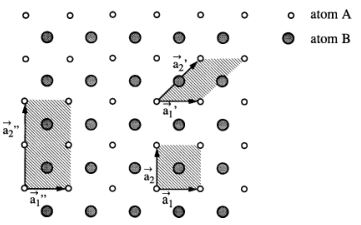
\includegraphics[clip,width=8cm]{7_1.JPG}
 \caption{単純単位胞当たり2つの異なる原子からなる基底を持つ2次元立方格子内の2つの単純単位胞(r.h.s)と1つの単純でない単位胞(l.h.s).}
 \label{7.1}
\end{figure}

\begin{figure}[tb]
 \centering
 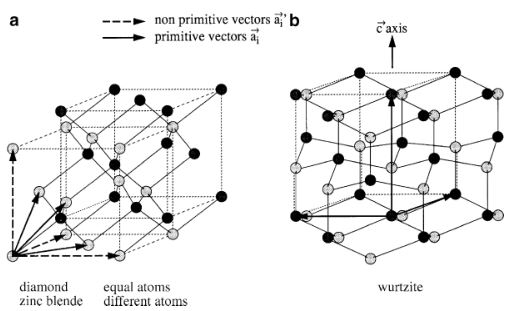
\includegraphics[clip,width=11cm]{7_2.JPG}
 \caption{ダイヤモンド及び閃亜鉛鉱型結晶構造(a)およびウルツ鉱型結晶構造(b)の単位胞(第1章[82L1]参照).}
 \label{7.2}
\end{figure}

ベクトル$R$は無限結晶において、並進群と呼ばれるアーベル群を形成している(26章)。単位胞中の原子の位置は、いわゆる基底によって与えられる。図7.1では基底は2つの原子からなっていて、一つの原子Aは(0,0)、一つの原子Bは($\frac{a}{2},\frac{a}{2}$)である。並進ベクトル$a_i$と基底は、結晶構造を記述するために必要なもののすべてである。

並進ベクトル$a_i$は、単純単位胞の中で原子がどこに位置するかについての情報を与える、抽象的な基底(並進不変点格子)を定義する。格子と基底は同時に結晶構造を定義する。

並進群のほかに、格子をそれ自身に変換するが、少なくとも一点が固定されたままである対称操作の、別の形がある。これらの対称操作はまた、点群と呼ばれる群を形成する。この群の要素はたとえば、鏡面での反射や、2倍・3倍・4倍・6倍対称の軸の周りの回転、あるいは原点を通る反転である。

さらに、回転面や鏡面を$a_i$の有理分数による並進と結びつけるようなねじれ面や滑る面が存在してもよい。抽象並進格子は、1つの三斜晶系、2つの単斜晶系、4つの斜方晶系、2つの正方晶系、3つの立方体、1つの三法晶系(菱面体)、1つの六方格子の14のブラベ格子に分類できる。

原子の位置と並進不変性を含める場合、無限の結晶をそれ自身に変換する対称操作の全ての組み合わせから、合計230個の空間群と呼ばれるものを見つける(そのうち73個は並進群と点群の積として記述することが出来る)。詳細は26章とその参考文献を参照のこと。半導体において最も重要な点群は、$O_h$(ダイヤモンド型結晶構造:Si,Ge,$\mathrm{Cu_2O}$,NaCl)、$T_d$(閃亜鉛鉱型結晶構造:ZnS,ZnSe,GaAs,InP,CuCl,AgBr)、そして$C_{6V}$(ウルツ鉱型結晶構造:ZnS,ZnO,CdS,GaN)である。図7.2にダイヤモンド、閃亜鉛鉱、ウルツ鉱の結晶構造を示す。ダイヤモンド結晶構造は、単位立方格子の空間対角線の$\frac{1}{4}$だけ移動した2つの面心立方格子(fcc)の格子点を占めるC原子からなっている。閃亜鉛鉱にとって、一つは同じ原理で、しかし、2つの副格子の一つは原子Aによって占められ、もう片方は原子Bに占められている。この状況は図7.2aに描かれている。もし、灰色と黒の"原子"が同一のものだったら、それはダイヤモンド構造と呼ばれる。図7.2aでは、点線の矢印の3つの単純でない並進ベクトル$a_i'$があり、それはfcc立方を定義している。実線の矢印は単純並進ベクトル$a_i$で、それは立方の角から始まり、角で交差する3つの面の中心に位置している3つの最も近い同一の原子を指している。ウルツ鉱結晶構造は、極性結晶学的なc軸を有する六方晶系である。この場合、なす角が$120^o$で等しい長さの、$\bm{a}$や$\bm{b}$とよく呼ばれる2つの単純並進ベクトルと、($\bm{c}$と呼ばれる)長さが異なり、$\bm{a}$と$\bm{b}$がなす平面に垂直な3番目のベクトルがある。ふつう、z軸はcと平行に選ばれる。3つのすべての場合において、一つの原子は、4つの最も近い原子によって四面体に囲まれている。閃亜鉛鉱とウルツ鉱の構造の違いは、次の最も近い原子の位置だけである。それゆえ、上記の化合物半導体のいくつかは、ZnS(これは2つのポリタイプを持つので悪名高い)、CdS、あるいはGaNの両方の構造で結晶化される。結晶モデルを使用して、これらの違いを結晶化することが推奨される。

半導体の化学結合は、$\mathrm{sp}^3$混成軌道による元素(C,Si,Ge)の共有結合であり、I\hspace{-1pt}I\hspace{-1pt}I-V、I\hspace{-1pt}$\mathrm{I}^{\mathrm{b}}$-V\hspace{-1pt}I、$\mathrm{I}^{\mathrm{b}}$-V\hspace{-1pt}I\hspace{-1pt}I結合となっていくにつれてイオン結合が強くなってゆき、最終的にはイオン結合が支配的になる。

逆格子について紹介したい。これは、実空間での格子と同じように、自身の基本並進ベクトル$\bm{b}_i$で定義される。$\bm{b}_i$は式(7.7)とインデックスの巡回置換で与えられ、$V_{\mathrm{uc}}$は式(7.8)で与えられる単位胞の体積である。

\begin{equation}
  \bm{b}_i=\frac{2\pi}{V_{\mathrm{uc}}}\bm{a}_2\bm{a}_3\tag{7.7}
\end{equation}

\begin{equation}
  V_{\mathrm{uc}}=\bm{a}_1(\bm{a}_2\times\bm{a}_3)\tag{7.8}
\end{equation}

逆格子空間の一般並進ベクトルはふつう$\bm{G}$で表される。

\begin{equation}
  \bm{G}=l_1\bm{b}_1+l_2\bm{b}_2+l_3\bm{b}_3\qquad l_i=0,\pm1,\pm2,...\qquad i=1,2,3\tag{7.9}
\end{equation}

複雑化なしに、逆格子のいくつかの性質や、逆格子と実格子の関係が得られる。

十分に滑らかで、式(7.6)で与えられる$\bm{R}$によって$f(\bm{r}+\bm{R})=f(\bm{r})$のように書かれる周期性を持つ、実空間におけるすべての周期関数は、全ての逆格子ベクトル$f(\bm{r})$の総和のフーリエ級数として書かれる。

\begin{equation}
  f(\bm{r})=\sum_{\bm{G}}f_{\bm{G}}\mathrm{e}^{\mathrm{i}\bm{Gr}}\qquad f_{\bm{G}}=V_{uc}^{-1}\int_{uc}f(\bm{r})\mathrm{e}^{\mathrm{i}\bm{Gr}}d\tau\tag{7.10}
\end{equation}

$\bm{R}$と$\bm{G}$の内積は常に式(7.11)を満たす。

\begin{equation}
  \bm{R}\cdot\bm{G}=2\pi m\qquad m=0,\pm1.\pm2,...\tag{7.11}
\end{equation}

結果として、周期格子で発生している効果を、実空間か逆空間のどちらかで記述することが選べる。後者は波数ベクトル$\bm{k}$または運動量$\hbar\bm{k}$に適した空間である。ある空間から別の空間への「並進」は、式(7.10)の3次元フーリエ級数によって与えられる。

結晶格子においては、空間における微小の並進に対する不変性はもはや無く、$a_i$の整数倍の並進に関する不変性のみがある。Noetherの定理による微小の並進の不変性から得られる運動量$\hbar\bm{k}$の保存則は、周期格子によって修正され、そのため$\hbar\bm{k}$は$b_i$の整数倍以下になるように保存される。すなわち、ある与えられたベクトル$\bm{k}$に逆格子ベクトル$\bm{G}$を加えることができる。

\begin{equation}
  \bm{k}\rightleftharpoons\bm{k}+\bm{G}\tag{7.12}
\end{equation}

これは、エネルギー保存則とともに、たとえば周期格子からのX線や中性子による回折のEwald構造の基礎を形どる重要なことである。

式(7.12)から、$\bm{k}$空間全体を考えなくてもよいのは明らかであるが、$\bm{b}_i$によって定義される「単位胞」による制限がある。単位胞の外のすべての$\bm{k}$ベクトルは、適切な$\bm{G}$を加えることによって単位胞の中へ移動される。ふつうそれは、図7.1あるいは7.2のように定義される単位胞の逆空間においては機能せず、2次元の場合のための、図7.3によって拡張されたもう一つの構築を用いる。一つは、逆格子上のある点(原点として選ばれた点)とほかのすべての点をつないだ線を二分するような垂直な平面を構築する。原点の周りを囲った図は、第1ブリルアンゾーンと呼ばれ、隣り合う同等の部分は第2ブリルアンゾーンを形成し、それが続いてゆく。全てのブリルアンゾーンは、2次元領域や3次元体積とそれぞれ等しい。全ての高次のブリルアンゾーンは、適切な$\bm{G}$ベクトルを加えることによって、第1ブリルアンゾーンに移動させられる。ブリルアンゾーンはまた、図7.1でなく図7.3によって構築されるある種類の基底のセルを形成する。
図7.3による、実空間に構築された最初のセルはWigner-Seitz胞として知られている。第1ブリルアンゾーンにおける高対称性の点や線の名前は図7.4に示されている。

\begin{figure}[tb]
 \centering
 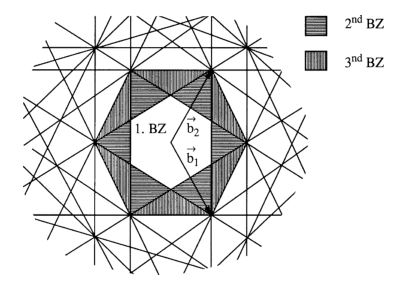
\includegraphics[clip,width=8.6cm]{7_3.JPG}
 \caption{2次元の逆格子における第1ブリルアンゾーン.}
 \label{7.3}
\end{figure}

\begin{figure}[tb]
 \centering
 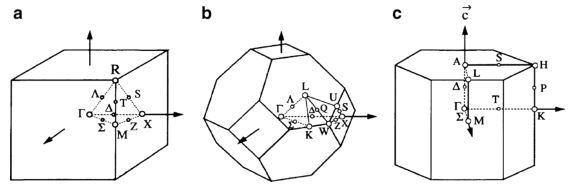
\includegraphics[clip,width=11cm]{7_4.JPG}
 \caption{単純立方格子(a)、ダイヤモンド型構造と閃亜鉛鉱型構造(b)(点群$O_h$、$T_d$)とウルツ鉱型構造(c)($C_{6V}$)の逆格子第1ブリルアンゾーン.高対称の点や方向の名前が示されている(第1章[82L1]による).}
 \label{7.4}
\end{figure}

単純な立方格子では
\begin{equation}
  \bm{a}_1=(a,0,0),\ \bm{a}_2=(0,a,0),\ \bm{a}_3=(0,0,a)\tag{7.13}
\end{equation}
であり、$\bm{b}_i$もまた直交し、
\begin{equation}
  \bm{b}_1=[\frac{2\pi}{a},0,0],\ \bm{b}_2=[0,\frac{2\pi}{a},0],\ \bm{b}_3=[0,0,\frac{2\pi}{a}]\tag{7.14}
\end{equation}
そして、第1ブリルアンゾーンは3次元すべての方向に広がる立方体である。
\begin{equation}
  -\frac{\pi}{a}\leq k_i\leq+\frac{\pi}{a},\ i=x,y,z\tag{7.15}
\end{equation}

今までの図や式において、簡単のために、式(7.15)のような第1ブリルアンゾーンの境界を与えるが、半導体を含むほとんどの固体は、今まで、あるいはこれから頻繁に説明する構造以外では、単純立方格子に結晶化されていない。例えば図7.9や図7.15、図7.17を見ること。

図7.4では、単純立方格子の第1ブリルアンゾーンや、いくつかの特別な点や方向の記法を含む単純単位胞を用いる点群$T_d$、$O_h$、$C_{6V}$が与えられている。第1ブリルアンゾーンの中心$\bm{k}=(0,0,0)$は$\Gamma$点と呼ばれ、他の高対称の点はラテンの大文字で、高対称の方向はギリシャ語の大文字でラベル付けされている。例えば、$T_d$対称においては、$\Gamma$点が$\Sigma$方向に離れた時、第1ブリルアンゾーンの境界の$K$点に到着する。

周期的な格子の励起の量$\hbar\bm{k}$は、たとえば光子や電子などの真空中の自由粒子の運動量$\bm{p}=\hbar\bm{k}$との違いを強調したい場合はふつう、準運動量と呼ばれる。ここで、式(7.12)とは異なり、逆格子ベクトルを加えることはできない。実際、あるケースから別のケースへ遷移することは可能である。格子定数がゼロになると、実空間において、系は無限小シフトを伴って並進分散を回復する。一方で、$\bm{b}_i$は式(7.7)の極限で無限大になり、第1ブリルアンゾーンは$\bm{k}$空間全体を満たすため、逆格子ベクトルは物理的な意味をなさなくなる。"準"運動量という用語のより詳細な議論は、7.6章や[98B1]の2章を参照のこと。

\subsection{ひもの振動}
7.3-7.6章では、[31F1]や多くの教科書で紹介されている方法で、格子振動と、その結果生じる量子やフォノンを扱う。つまり、均質なひもから始めて、単原子や二原子鎖に進み、最後に3次元固体を扱う。

最初に、図7.5で概略的に示されているように、準1次元ひもを考える。それに沿って、縦波と横波の2種類の波が伝搬できる。伸びる方向は、伝搬方向に対して垂直な、つまりx-y平面か、平行、つまりz方向、のいずれかである。後者から考える。ひもの質量密度を$\rho$、断面積を$A$、平衡位置からの$z$でのひもの無限小片$\mathrm{d}z$の伸びを$u(z)$とする。このとき、ニュートンの運動方程式は式(7.16)のようになる。

\begin{equation}
  \mathrm{d}m\frac{\partial^2u}{\partial t^2}=\rho A\cdot\mathrm{d}z\cdot\frac{\partial^2u}{\partial t^2}=F\tag{7.16}
\end{equation}

\begin{figure}[tb]
 \centering
 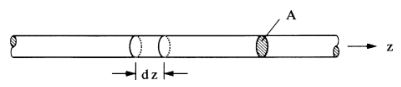
\includegraphics[clip,width=8cm]{7_5.JPG}
 \caption{式(7.19)の導出を説明するモデルとしてのひも.}
 \label{7.5}
\end{figure}

力$F$は弾性率$E$と次のような関係がある。

\begin{equation}
  F=A\cdot E\frac{\partial^2u}{\partial z^2}\tag{7.17}
\end{equation}

式(7.17)における2階微分の出現は、フックの法則に注意して、何人かの学生に驚きを与える。しかし、応力$\sigma$は式(7.18)によって与えられると考えなければならない。

\begin{equation}
  \sigma(z)=E\frac{\partial u}{\partial z}\tag{7.18}
\end{equation}

応力が長さ$\mathrm{d}z$の微小要素の両端で同じならば、$z$と$z+\mathrm{d}z$で生じる力は互いにゼロに補正される。復元力$F$はそれゆえ、式(7.17)のように$\mathrm{d}\sigma/\mathrm{d}z$で与えられる。

式(7.16)と(7.17)の組み合わせから、基本的な調和波の式を導ける。

\begin{equation}
  \rho\frac{\partial^2u}{\partial t^2}=E\frac{\partial^2u}{\partial z^2}\tag{7.19}
\end{equation}
式(7.19)の解は次のようになり、

\begin{equation}
  u=u_0\mathrm{exp}[\mathrm{i}(kz-\omega t)]\tag{7.20}
\end{equation}
平面波において、縦波の分散関係が得られる。

\begin{equation}
  \omega_L=(E/\rho)^{1/2}k\tag{7.21}
\end{equation}

これは、図7.6に見えるように、線形関係である。結果として、位相と群速度は一定で、等しく、すなわち式(2.13)のようになる。

\begin{equation}
  v_{\mathrm{ph}^L}=v_{\mathrm{g}^L}=(E/\rho)^{1/2}\tag{7.22}
\end{equation}

\begin{figure}[tb]
 \centering
 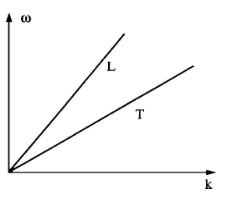
\includegraphics[clip,width=5cm]{7_6.JPG}
 \caption{均質なひも上の波の分散関係.}
 \label{7.6}
\end{figure}

2重縮退の横波を考えると、、同様の方法で、以下のことがわかる。

\begin{equation}
  \omega_T=(G/\rho)^{1/2}\tag{7.23}
\end{equation}

\begin{equation}
  v_{\mathrm{ph}^T}=v_{\mathrm{g}^T}=(G/\rho)^{1/2}\tag{7.24}
\end{equation}
ここで、$G$はせん断係数あるいはねじれ係数である。

弾性理論で式(7.25)がよく知られているため、式(7.26)がわかる。

\begin{equation}
  G\leq E\tag{7.25}
\end{equation}

\begin{equation}
  v_{ph}^T\leq v_{ph}^L\tag{7.26}
\end{equation}

これは式(4.28)と同等の結果である。

\end{document}
